% Poster variant (larger type). Scenario results by category (docs/evaluation_results.json, demo mode, 1 run, and
% docs/evaluation_results_llm.json, LLM mode, 3 runs: a scenario counts as passed in LLM mode only
% when it passed in all 3 runs, consistency 1.0). Core: 23 of 23 in both modes. Known-limitation
% cases: demo 1 of 2, LLM 2 of 2.
\documentclass[border=3pt]{standalone}
% Shared style of every Roameo figure (the deck and the poster).
% Type is near-black and grey on white. Teal, the colour of the app, is the brand and the system.
% One warm accent marks tension only (the budget gap, the over-budget plan). Green marks only a
% confirmed result: a human approval or a passed test. Thin rules, no shadows, no gradients.
\usepackage[T1]{fontenc}
\usepackage[scaled]{helvet}
\renewcommand{\familydefault}{\sfdefault}
\usepackage{tikz}
\usepackage{pgfplots}
\pgfplotsset{compat=1.18}
\usepackage{fontawesome5}
\hyphenpenalty=10000
\exhyphenpenalty=10000
\usetikzlibrary{arrows.meta,positioning,calc,fit,backgrounds,shapes.callouts,shapes.misc}

% Colours
\definecolor{primary}{HTML}{0F766E}   % Roameo teal: the system, the agents
\definecolor{primarysoft}{HTML}{E3F1EF}
\definecolor{accent}{HTML}{C2410C}    % tension only: the budget gap
\definecolor{accentsoft}{HTML}{FBE9E1}
\definecolor{ok}{HTML}{4D7C0F}        % a confirmed result: approval, a passed test
\definecolor{oksoft}{HTML}{EDF3E1}
\definecolor{ink}{HTML}{1F1F1F}
\definecolor{muted}{HTML}{5F6368}
\definecolor{quiet}{HTML}{9A9A9A}
\definecolor{rulegrey}{HTML}{C4C4C4}
\definecolor{gridgrey}{HTML}{E4E4E4}
\definecolor{faint}{HTML}{F4F4F4}

\tikzset{
  >={Stealth[length=2.4mm,width=1.8mm]},
  every picture/.style={line cap=butt, line join=miter},
  % text styles
  hd/.style={font=\bfseries, text=ink, align=left},
  sub/.style={text=muted, align=left},
  % shapes: 2 pt corners, thin rules
  card/.style={draw=rulegrey, line width=0.5pt, fill=white, rounded corners=2pt, inner sep=5pt, align=left, text=ink},
  sys/.style={draw=primary, line width=0.8pt, fill=white, rounded corners=2pt, inner sep=5pt, align=center, text=ink},
  sysfill/.style={draw=primary, line width=0.8pt, fill=primary, rounded corners=2pt, inner sep=5pt, align=center, text=white},
  code/.style={draw=ink, line width=0.8pt, fill=faint, rounded corners=2pt, inner sep=5pt, align=center, text=ink},
  warm/.style={draw=accent, line width=0.8pt, fill=accentsoft, rounded corners=2pt, inner sep=5pt, align=left, text=ink},
  receipt/.style={draw=ok, line width=0.8pt, fill=oksoft, rounded corners=2pt, inner sep=5pt, align=left, text=ink},
  planned/.style={draw=muted, line width=0.6pt, dash pattern=on 3pt off 2pt, fill=white, rounded corners=2pt, inner sep=5pt, align=left, text=muted},
  % chat bubbles: the traveller in teal, the app in light grey
  saybubble/.style={fill=primary, text=white, rounded corners=6pt, inner sep=5pt, align=left},
  appbubble/.style={fill=faint, text=ink, rounded corners=6pt, inner sep=5pt, align=left},
  chip/.style={draw=rulegrey, line width=0.5pt, fill=white, rounded corners=7pt, inner sep=4pt, text=ink},
  % connectors
  link/.style={->, draw=muted, line width=0.6pt},
  syslink/.style={->, draw=primary, line width=0.9pt},
  oklink/.style={->, draw=ok, line width=0.9pt},
  warmlink/.style={->, draw=accent, line width=0.9pt},
  nextlink/.style={->, draw=muted, line width=0.6pt, dash pattern=on 3pt off 2pt},
}

% Charts: a real axis, few light gridlines, no frame on the top and right.
\pgfplotsset{
  roameo/.style={
    axis line style={draw=muted, line width=0.5pt},
    tick style={draw=muted, line width=0.5pt},
    major tick length=3pt,
    tick label style={text=ink, /pgf/number format/assume math mode=true},
    label style={text=ink},
    title style={font=\bfseries, text=ink},
    grid style={draw=gridgrey, line width=0.4pt},
    every axis plot/.append style={line width=0.6pt},
    legend style={draw=none, fill=none, text=ink},
    legend cell align=left,
  },
}

\begin{document}
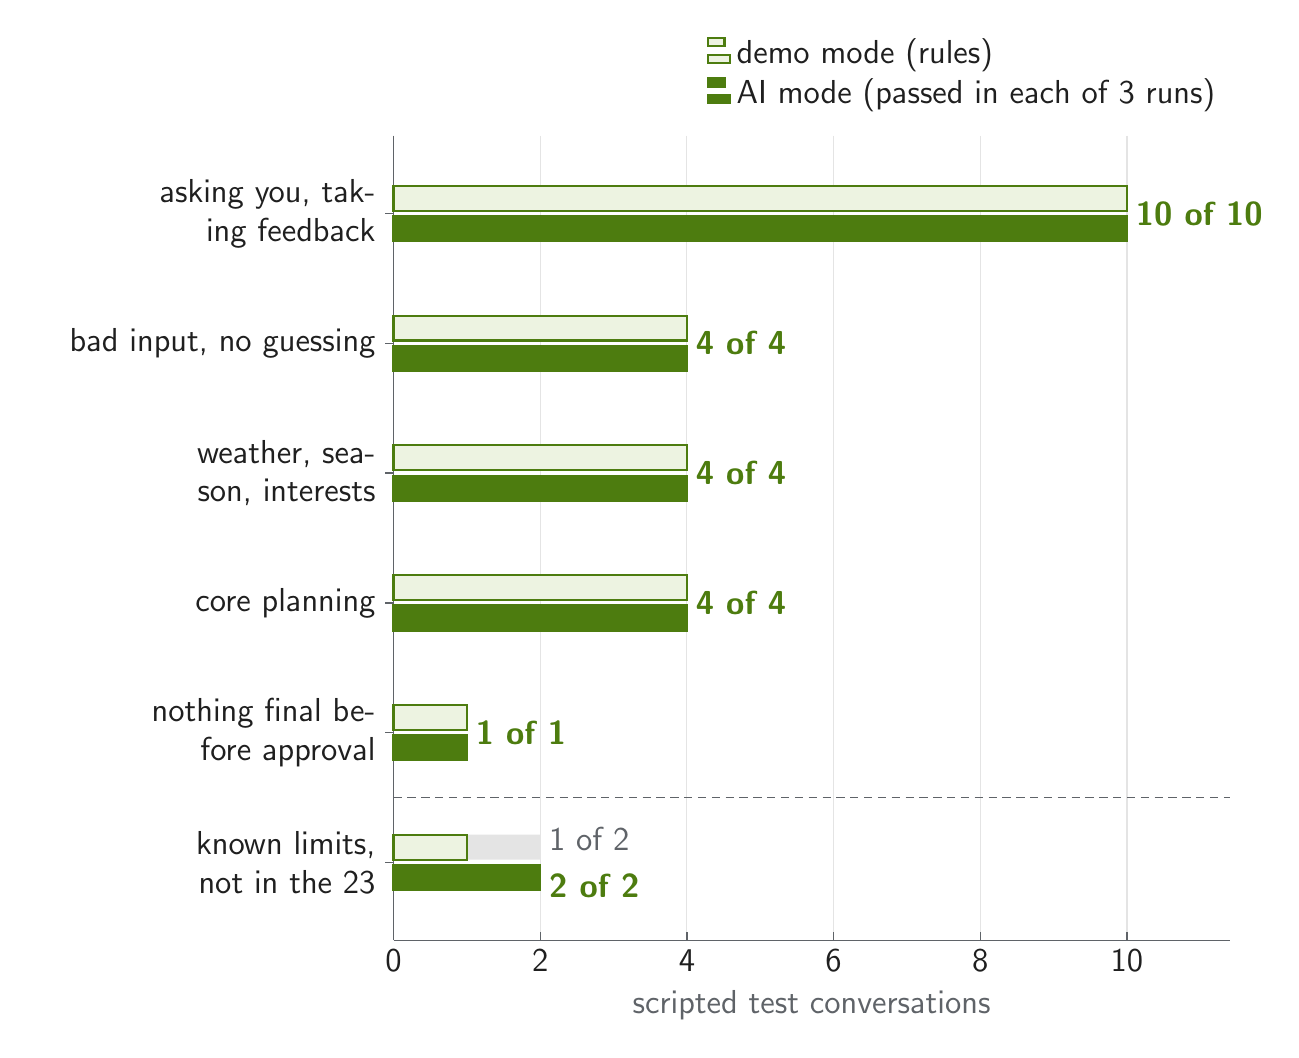
\begin{tikzpicture}[font=\large]
  \begin{axis}[roameo,
    xbar, width=12.2cm, height=11.8cm,
    bar width=9pt,
    xmin=0, xmax=11.4,
    axis x line*=bottom, axis y line*=left,
    y dir=reverse,
    ytick={1,...,6},
    yticklabels={{asking you, taking feedback}, {bad input, no guessing}, {weather, season, interests}, {core planning}, {nothing final before approval}, {known limits, not in the 23}},
    yticklabel style={font=\large, text width=4.3cm, align=right},
    ymin=0.4, ymax=6.6,
    xtick={0,2,...,10},
    xmajorgrids,
    xlabel={scripted test conversations}, xlabel style={font=\large, text=muted},
    legend style={at={(1.0,1.02)}, anchor=south east, legend columns=1, font=\large, /tikz/every even column/.append style={column sep=10pt}},
    clip=false,
  ]
    % ghost bars: how many scenarios there are
    \addplot[draw=none, fill=gridgrey, bar shift=5.5pt, forget plot] coordinates {(10,1) (4,2) (4,3) (4,4) (1,5) (2,6)};
    \addplot[draw=none, fill=gridgrey, bar shift=-5.5pt, forget plot] coordinates {(10,1) (4,2) (4,3) (4,4) (1,5) (2,6)};
    % passed
    \addplot[draw=ok, fill=oksoft, line width=0.8pt, bar shift=5.5pt] coordinates {(10,1) (4,2) (4,3) (4,4) (1,5) (1,6)};
    \addplot[draw=ok, fill=ok, line width=0.8pt, bar shift=-5.5pt] coordinates {(10,1) (4,2) (4,3) (4,4) (1,5) (2,6)};
    \draw[draw=muted, line width=0.6pt, dash pattern=on 3pt off 2pt] (axis cs:0,5.5) -- (axis cs:11.4,5.5);
    \legend{demo mode (rules), AI mode (passed in each of 3 runs)}
    \node[anchor=west, font=\large\bfseries, text=ok, inner sep=3pt] at (axis cs:10,1) {10 of 10};
    \node[anchor=west, font=\large\bfseries, text=ok, inner sep=3pt] at (axis cs:4,2) {4 of 4};
    \node[anchor=west, font=\large\bfseries, text=ok, inner sep=3pt] at (axis cs:4,3) {4 of 4};
    \node[anchor=west, font=\large\bfseries, text=ok, inner sep=3pt] at (axis cs:4,4) {4 of 4};
    \node[anchor=west, font=\large\bfseries, text=ok, inner sep=3pt] at (axis cs:1,5) {1 of 1};
    \node[anchor=west, font=\large, text=muted, inner sep=3pt] at (axis cs:2,5.82) {1 of 2};
    \node[anchor=west, font=\large\bfseries, text=ok, inner sep=3pt] at (axis cs:2,6.18) {2 of 2};
  \end{axis}
\end{tikzpicture}
\end{document}
